\documentclass{report}
\usepackage{geometry}
\usepackage{paralist}
\usepackage{scalerel,amssymb}
\usepackage{tikz}
\usetikzlibrary{positioning}
\usepackage{amsmath}
\usepackage{array}
\usepackage{nccmath}

\usepackage{fancyhdr}
\fancyhead[L]{\LARGE Modal Logic \\
\Large Exercise 01}
\fancyhead[R]{13-123-922 \\
Elias \textsc{Wipfli} \\
16-124-836 \\
Marcel \textsc{Zauder}}
\renewcommand{\headrulewidth}{0.4pt}
\fancyfoot[C]{\thepage}
\renewcommand{\footrulewidth}{0.4pt}

\usepackage{hyperref}

\begin{document}
	\pagestyle{fancy}
	\hfill
	
	\section*{Problem 1.1}
	\subsection*{1.1.1 $M, w_1 \Vdash q$}
	\begin{enumerate}[]
		\item $M, w \Vdash q$ iff $w \in V(q)$ but $w_1 \not \in V(q)$, so it is \textsc{False}.
	\end{enumerate}
	\subsection*{1.1.2 $M, w_3 \Vdash \neg q$}
	\begin{enumerate}[]
		\item $M, w \Vdash \neg q$ iff $w \in V(\neg q)$. $w_3 \in V(\neg q)$, so it is \textsc{True}.
	\end{enumerate}
	\subsection*{1.1.3 $M, w_1 \Vdash p \vee q$}
	\begin{enumerate}[]
		\item $M, w \Vdash p \vee q$ iff $w \in V(p)$ \textsc{or} $w \in V(q)$. $w_1 \in V(p)$, so it is \textsc{True}.
	\end{enumerate}
	\subsection*{1.1.4 $M, w_1 \Vdash \square (p \vee q)$}
	\begin{align*}
		M, w_1 \Vdash \square (p \vee q) \ & \Rightarrow \ \forall v \in V : Rw_1v \Rightarrow M, v \Vdash (p \vee q) \\
		& \Rightarrow \ \forall v \in V : Rw_1v \Rightarrow v \in V(p) \textsc{ or } v \in V(q) \\
		& \textsc{because } w_3 \in V \textit{ with } Rw_1w_3, \textit{ but }w_3 \not \in V(p) \textsc{ and } w_3 \not \in V(q) \\
		& \Rightarrow \ \textsc{False}
	\end{align*}
	\subsection*{1.1.5 $M, w_3 \Vdash \square q$}
	\begin{align*}
		M, w_3 \Vdash \square q \ & \Rightarrow \ \underbrace{\forall v \in V : Rw_1v}_{\textsc{False}} \Rightarrow M,v \Vdash q \\
		& \textsc{because } \textit{the left side of the statement is \textsc{False} everything can follow} \\
		& \Rightarrow \ \textsc{True}
	\end{align*}
	\subsection*{1.1.6 $M, w_3 \Vdash \square \bot$}
	\begin{align*}
		M, w_3 \Vdash \square \bot \ & \Rightarrow \ \underbrace{\forall v \in V : Rw_1v}_{\textsc{False}} \Rightarrow M,v \Vdash \bot \\
		& \textsc{because } \textit{the left side of the statement is \textsc{False} everything can follow} \\
		& \Rightarrow \ \textsc{True}
	\end{align*}
	\subsection*{1.1.7 $M, w_1 \Vdash \diamond q$}
	\begin{align*}
		M, w_1 \Vdash \diamond q \ & \Rightarrow \ \exists v \in V : Rw_1v \Rightarrow M,v \Vdash q \\
		& \Rightarrow \ \exists v \in V : Rw_1v \Rightarrow v \in V(q) \\
		& \textsc{because } w_2 \in V : Rw_1w_2 \textit{ and } w_2 \in V(q) \\
		& \Rightarrow \ \textsc{True}
	\end{align*}
	\subsection*{1.1.8 $M, w_1 \Vdash \square q$}
	\begin{align*}
		M, w_1 \Vdash \square q \ & \Rightarrow \ \forall v \in V : Rw_1v \Rightarrow M, v \Vdash q \\
		& \Rightarrow \ \forall v \in V : Rw_1v \Rightarrow v \in V(q) \\
		& \textsc{because } w_3 \in V : Rw_1w_3, \textit{ but } w_3 \not \in V(q) \\
		& \Rightarrow \ \textsc{False}
	\end{align*}
	\subsection*{1.1.9 $M, w_1 \Vdash \neg \square \square \neg q$}
	\begin{align*}
		M, w_1 \Vdash \neg \square \square \neg q \ & \Rightarrow \ \nexists v_1 \in V : Rw_1v_1 \Rightarrow M, v_1 \Vdash \square \neg q \\
		& \Rightarrow \ \nexists v_1 \in V : Rw_1v_1 \Rightarrow \underbrace{\forall v_2 \in V : Rv_1v_2}_{\textsc{False}} \Rightarrow M, v_2 \Vdash \neg q \\
		& \Rightarrow \ \nexists v_1 \in V : Rw_1v_1 \Rightarrow \textsc{ True} \\
		& \Rightarrow \ \textsc{False}
	\end{align*}
	
	\section*{Problem 1.5}
		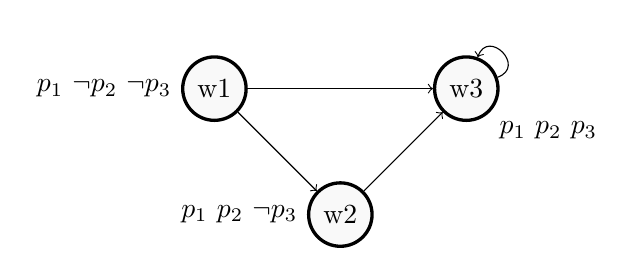
\begin{tikzpicture}[
			roundnode/.style={circle, draw=black, fill=gray!5, very thick, minimum size=7mm},
		]
		
			%Nodes
			\node[roundnode, label=left: $p_1 \ \neg p_2 \ \neg p_3$]		(w1)	{w1};
			\node[roundnode, label=left: $p_1 \ p_2 \ \neg p_3$]		(w2)	[below right=of w1]	{w2};
			\node[roundnode, label=below right: $p_1 \ p_2 \ p_3$]		(w3)	[above right=of w2]	{w3};
		
			%Lines
			\draw[->]	(w1.-45) -- (w2.135);
			\draw[->]	(w2.45) -- (w3.-135);
			\draw[->]	(w1.east) -- (w3.west);
			\draw[->]	(w3) to [out=20,in=70,loop,looseness=2.8] (w3);
		
		\end{tikzpicture}
		\subsection*{1.5.1 $p \rightarrow \square p$}
		\begin{enumerate}[]
			\item \textit{For} $w_1$:
			\begin{enumerate}[]
				\item $M, w_1 \Vdash p_1 \rightarrow \diamond p_1$ holds, because $w_2$, $w_3$ have $p_1$.
				\item $M, w_1 \Vdash p_2 \rightarrow \diamond p_2$ holds, because $M, w_1 \not \Vdash p_2$.
				\item $M, w_1 \Vdash p_3 \rightarrow \diamond p_3$ holds, because $M, w_1 \not \Vdash p_3$.
			\end{enumerate}
			\item \textit{For} $w_2$:
			\begin{enumerate}[]
				\item $M, w_2 \Vdash p_1 \rightarrow \diamond p_1$ holds, because $w_3$ has $p_1$.
				\item $M, w_2 \Vdash p_2 \rightarrow \diamond p_2$ holds, because $w_3$ has $p_2$.
				\item $M, w_21 \Vdash p_3 \rightarrow \diamond p_3$ holds, because $M, w_2 \not \Vdash p_3$.
			\end{enumerate}
			\item \textit{For} $w_3$:
			\begin{enumerate}[]
				\item $M, w_3 \Vdash p_1 \rightarrow \diamond p_1$ holds, because we have $Rw_3w_3$ with $M, w_3 \Vdash p_1$.
				\item Same for $p_2$ and $p_3$.
			\end{enumerate}
			\item $\Rightarrow$ $p \rightarrow \diamond p$ holds for all $w \in W$. 
		\end{enumerate}
		\subsection*{1.5.2 $A \rightarrow \diamond A$}
		\begin{enumerate}[]
			\item $A = ((p_2 \rightarrow \bot ) \wedge (p_3 \rightarrow \bot))$
			\item Then $M, w_1 \Vdash A$ holds \\
			but $M, w_2 \not \Vdash A$ and $M, w_3 \not \Vdash A$.
			\item Therefore $A \rightarrow \square A$ is not \textsc{True}.
		\end{enumerate}
		\subsection*{1.5.3 $\square p \rightarrow p$}
		\begin{enumerate}[]
			\item does not hold because: \\
			$M, w_1 \Vdash \square p_2$ holds but $M, w_1 \not \Vdash p_2$
		\end{enumerate}
		\subsection*{1.5.4 $\neg p \rightarrow \diamond \square p$}
		\begin{enumerate}[]
			\item \textit{For} $w_1$:
			\begin{enumerate}[]
				\item $M, w_1 \Vdash \neg p_1 \rightarrow \diamond \square p_1$ holds, because $M, w_1 \not \Vdash \neg p_1$.
				\item $M, w_1 \Vdash \neg p_2 \rightarrow \diamond \square p_2$ holds, because we have $Rw_1w_2$ with $M,w_2 \Vdash \square p_2$, because we have $Rw_2w_3$ with $M,w_3 \Vdash p_2$.
				\item $M, w_1 \Vdash \neg p_3 \rightarrow \diamond \square p_3$ holds, because we have $Rw_1w_2$ with $M,w_2 \Vdash \square p_3$, because we have $Rw_2w_3$ with $M,w_3 \Vdash p_3$.
			\end{enumerate}
			\item \textit{For} $w_2$:
			\begin{enumerate}[]
				\item $M, w_2 \Vdash \neg p_1 \rightarrow \diamond \square p_1$ holds, because $M, w_2 \not \Vdash \neg p_1$.
				\item $M, w_2 \Vdash \neg p_2 \rightarrow \diamond \square p_2$ holds, because $M, w_2 \not \Vdash \neg p_2$.
				\item $M, w_2 \Vdash \neg p_3 \rightarrow \diamond \square p_3$ holds, because we have $Rw_2w_3$ with $M,w_3 \Vdash \square p_3$, because we have $Rw_3w_3$ with $M,w_3 \Vdash p_3$.
			\end{enumerate}
			\item \textit{For} $w_3$:
			\begin{enumerate}[]
				\item $M, w_3 \Vdash \neg p_1 \rightarrow \diamond \square p_1$ holds, because $M, w_3 \not \Vdash \neg p_1$.
				\item $M, w_3 \Vdash \neg p_2 \rightarrow \diamond \square p_2$ holds, because $M, w_3 \not \Vdash \neg p_2$.
				\item $M, w_3 \Vdash \neg p_3 \rightarrow \diamond \square p_3$ holds, because $M, w_3 \not \Vdash \neg p_3$.
			\end{enumerate}
			\item $\Rightarrow$ $\neg p \rightarrow \diamond \square p$ holds for all $w \in W$. 
		\end{enumerate}
		\subsection*{1.5.5 $\diamond \square A$}
		\begin{enumerate}[]
			\item $A = \neg p_1$
			\item $M, w_1 \Vdash \diamond \square \neg p_1$ does not hold because this implies $Rw_1w_2$ with $M, w_2 \Vdash \square \neg p_1$ but we have $Rw_2w_3$ with $M, w_3 \not \Vdash \neg p_1$.
		\end{enumerate}
		\subsection*{1.5.6 $\square \diamond p$}
		\begin{enumerate}[]
			\item \textit{For} $w_1$:
			\begin{enumerate}[]
				\item $M, w_1 \Vdash \square \diamond p_1$ holds because:
				\begin{enumerate}[]
					\item For $Rw_1w_2$ with $M,w_2 \Vdash \diamond p_1$ we have $Rw_2w_3$ with $M, w_3 \Vdash p_1$
					\item For $Rw_1w_3$ with $M,w_3 \Vdash \diamond p_1$ we have $Rw_3w_3$ with $M, w_3 \Vdash p_1$
				\end{enumerate}
				\item $M, w_1 \Vdash \square \diamond p_2$ holds because:
				\begin{enumerate}[]
					\item For $Rw_1w_2$ with $M,w_2 \Vdash \diamond p_2$ we have $Rw_2w_3$ with $M, w_3 \Vdash p_2$
					\item For $Rw_1w_3$ with $M,w_3 \Vdash \diamond p_2$ we have $Rw_3w_3$ with $M, w_3 \Vdash p_2$
				\end{enumerate}
				\item $M, w_1 \Vdash \square \diamond p_3$ holds because:
				\begin{enumerate}[]
					\item For $Rw_1w_2$ with $M,w_2 \Vdash \diamond p_3$ we have $Rw_2w_3$ with $M, w_3 \Vdash p_3$
					\item For $Rw_1w_3$ with $M,w_3 \Vdash \diamond p_3$ we have $Rw_3w_3$ with $M, w_3 \Vdash p_3$
				\end{enumerate}
			\end{enumerate}
			\item \textit{For} $w_2$:
			\begin{enumerate}[]
				\item $M, w_2 \Vdash \square \diamond p_1$ holds because:
				\begin{enumerate}[]
					\item For $Rw_2w_3$ with $M,w_3 \Vdash \diamond p_1$ we have $Rw_3w_3$ with $M, w_3 \Vdash p_1$
				\end{enumerate}
				\item $M, w_2 \Vdash \square \diamond p_2$ holds because:
				\begin{enumerate}[]
					\item For $Rw_2w_3$ with $M,w_3 \Vdash \diamond p_2$ we have $Rw_3w_3$ with $M, w_3 \Vdash p_2$
				\end{enumerate}
				\item $M, w_2 \Vdash \square \diamond p_3$ holds because:
				\begin{enumerate}[]
					\item For $Rw_2w_3$ with $M,w_3 \Vdash \diamond p_3$ we have $Rw_3w_3$ with $M, w_3 \Vdash p_3$
				\end{enumerate}
			\end{enumerate}
			\item \textit{For} $w_3$:
			\begin{enumerate}[]
				\item $M, w_3 \Vdash \square \diamond p_1$ holds because:
				\begin{enumerate}[]
					\item For $Rw_3w_3$ with $M,w_3 \Vdash \diamond p_1$ we have $Rw_3w_3$ with $M, w_3 \Vdash p_1$
				\end{enumerate}
				\item $M, w_3 \Vdash \square \diamond p_2$ holds because:
				\begin{enumerate}[]
					\item For $Rw_3w_3$ with $M,w_3 \Vdash \diamond p_2$ we have $Rw_3w_3$ with $M, w_3 \Vdash p_2$
				\end{enumerate}
				\item $M, w_3 \Vdash \square \diamond p_3$ holds because:
				\begin{enumerate}[]
					\item For $Rw_3w_3$ with $M,w_3 \Vdash \diamond p_3$ we have $Rw_3w_3$ with $M, w_3 \Vdash p_3$
				\end{enumerate}
			\end{enumerate}
			$\Rightarrow$ $\square \diamond p$ holds for all $w \in W$. 
		\end{enumerate}
	
	\section*{Problem 1.6}
	Show that the following are valid:
	\subsection*{1.6.1 $\models \square p \rightarrow \square(q \rightarrow p)$}
	We will show that the negation of this statement is always \textsc{False}:
	\begin{center}
		\begin{tabular}{ccccc}
			\multicolumn{5}{c}{$\neg (\square p \rightarrow \square (q \rightarrow p))$} \\ \hline
			$\square p$ & $\mid$ & \multicolumn{3}{c}{$\neg (\square (q \rightarrow p))$} \\ \cline{1-1} \cline{3-5}
			$p$ & & \multicolumn{3}{c}{$\neg (q \rightarrow p)$} \\ \cline{3-5}
			& & $q$ & $\mid$ & $\neg p$
		\end{tabular}
	\end{center}
	Because we get $p$ and $\neg p$ to be \textsc{True} we can conclude that our assumption must be \textsc{False}.
	\subsection*{1.6.2 $\models \square \neg \bot$}
	We will show that the negation of this statement is always \textsc{False}:
	\begin{center}
		\begin{tabular}{c}
			$\neg (\square \neg \bot)$ \\ \hline
			$\neg \neg \bot $ \\ \hline
			$\bot $
		\end{tabular}
	\end{center}
	It is obvious that this statement is always \textsc{False}.
	\subsection*{1.6.3 $\models \square p \rightarrow(\square q \rightarrow \square p)$}
	We will show that the negation of this statement is always \textsc{False}:
	\begin{center}
		\begin{tabular}{ccccc}
			\multicolumn{5}{c}{$\neg (\square p \rightarrow (\square q \rightarrow \square p))$} \\ \hline
			$\square p$ & $\mid$ & \multicolumn{3}{c}{$\neg (\square q \rightarrow \square p)$} \\ \cline{1-1} \cline{3-5}
			$p$ & & $\square q$ & $\mid$ & $\neg \square p$ \\ \cline{3-3} \cline{5-5}
			& & $q$ & & $\neg p$
		\end{tabular}
	\end{center}
	Because We get $p$ and $\neg p$ to be \textsc{True} we can conclude that our assumption must be \textsc{False}.
	\section*{Problem 1.10}
	Show that none of the following formulas are valid:
	\subsection*{1.10.1 $\square p \rightarrow \diamond p$}
		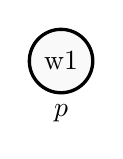
\begin{tikzpicture}[
			roundnode/.style={circle, draw=black, fill=gray!5, very thick, minimum size=7mm},
		]
		
			%Nodes
			\node[roundnode, label=below: $p$]		(w1)				{w1};
		
			%Lines
		
		\end{tikzpicture} \\
		In this model $\square p$ is clearly \textsc{True}. But because there is no world that can be reached from $w_1$ $\diamond p$ is \textsc{False} and therefore $\square p \rightarrow \diamond p$ is also \textsc{False}.
	\subsection*{1.10.2 $\square p \rightarrow p$}
		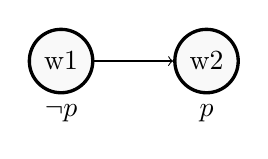
\begin{tikzpicture}[
			roundnode/.style={circle, draw=black, fill=gray!5, very thick, minimum size=7mm},
		]
		
			%Nodes
			\node[roundnode, label=below: $\neg p$]	(w1)				{w1};
			\node[roundnode, label=below: $p$]		(w2)[right=of w1]	{w2};
		
			%Lines
			\draw[->]	(w1.east) -- (w2.west);
		
		\end{tikzpicture} \\
		In this model $\square p$ is clearly \textsc{True} in all worlds. But $p$ is not \textsc{True} in all worlds. Therefore $\square p \rightarrow p$ is \textsc{False}.
	\subsection*{1.10.3 $p \rightarrow \square \diamond p$}
		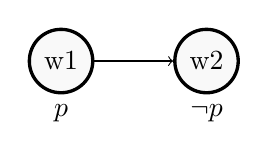
\begin{tikzpicture}[
			roundnode/.style={circle, draw=black, fill=gray!5, very thick, minimum size=7mm},
		]
		
			%Nodes
			\node[roundnode, label=below: $p$]		(w1)				{w1};
			\node[roundnode, label=below: $\neg p$]	(w2)[right=of w1]	{w2};
		
			%Lines
			\draw[->]	(w1.east) -- (w2.west);
		
		\end{tikzpicture} \\
		In this model  is $p$ is clearly \textsc{True}. But world $w_2$ has no following world and therefore $\diamond p$ is \textsc{False} and therefore the statement is not valid.
	\subsection*{1.10.4 $\square p \rightarrow \square \square p$}
		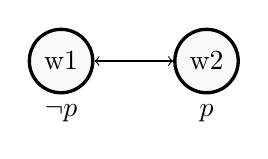
\begin{tikzpicture}[
			roundnode/.style={circle, draw=black, fill=gray!5, very thick, minimum size=7mm},
		]
		
			%Nodes
			\node[roundnode, label=below: $\neg p$]		(w1)				{w1};
			\node[roundnode, label=below: $p$]		(w2)[right=of w1]	{w2};
		
			%Lines
			\draw[<->]	(w1.east) -- (w2.west);
		
		\end{tikzpicture} \\
		In this model $\square p$ is \textsc{True} but we cannot reach a world from $w_2$ where $p$ is \textsc{True} and therefore $\square \square p$ is \textsc{False}.
	\subsection*{1.10.5 $\diamond p \rightarrow \square \diamond p$}
		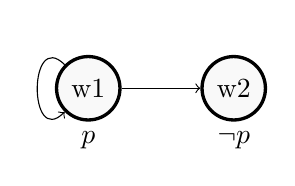
\begin{tikzpicture}[
			roundnode/.style={circle, draw=black, fill=gray!5, very thick, minimum size=7mm},
		]
		
			%Nodes
			\node[roundnode, label=below: $p$]		(w1)				{w1};
			\node[roundnode, label=below: $\neg p$]		(w2)[right=of w1]	{w2};
		
			%Lines
			\draw[->]	(w1.east) -- (w2.west);
			\draw[->]	(w1) to [out=135,in=225,loop,looseness=2.8] (w1);
		
		\end{tikzpicture} \\
		In this model $\diamond p$ is \textsc{True} because we can reach $w_1$ from $w_1$. But there is no following world for $w_2$ and therefore $\square \diamond p$ is \textsc{False}.
	
	\section*{Problem 1.13}
	For each of the following schemes find a model M such that every instance of the formula is \textsc{true} in M:
	\subsection*{1.13.1 $p \rightarrow \diamond \diamond p$}
		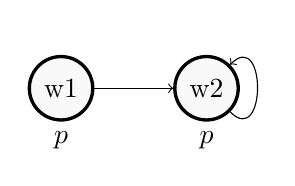
\begin{tikzpicture}[
			roundnode/.style={circle, draw=black, fill=gray!5, very thick, minimum size=7mm},
		]
		
			%Nodes
			\node[roundnode, label=below: $p$]		(w1)				{w1};
			\node[roundnode, label=below: $p$]		(w2)[right=of w1]	{w2};
		
			%Lines
			\draw[->]	(w1.east) -- (w2.west);
			\draw[->]	(w2) to [out=315,in=45,loop,looseness=2.8] (w2);
		
		\end{tikzpicture}
	\subsection*{1.13.2 $\diamond p \rightarrow \square p$}
		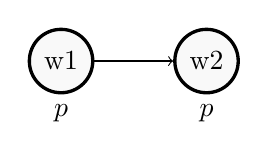
\begin{tikzpicture}[
			roundnode/.style={circle, draw=black, fill=gray!5, very thick, minimum size=7mm},
		]
		
			%Nodes
			\node[roundnode, label=below: $p$]		(w1)				{w1};
			\node[roundnode, label=below: $p$]		(w2)[right=of w1]	{w2};
		
			%Lines
			\draw[->]	(w1.east) -- (w2.west);
		
		\end{tikzpicture}
	
	\section*{Problem 1.14}
	Show that $\square (A \wedge B) \models \square A$. \\
	Let M = $\langle W,R,V \rangle$ be a model and $w \in W$. Then we have:
	\begin{align*}
		\square (A \wedge B) \models \square A \ & \Rightarrow \ \forall w \in W: M,w \Vdash \square (A \wedge B) \\
		& \Rightarrow \ \forall w' \in W: Rww' \Rightarrow M,w' \Vdash (A \wedge B) \\
		& \Rightarrow \ w' \in V(A \wedge B) \\
		& \Rightarrow \ w' \in V(A) \textsc{ and } w' \in V(B) \\
		& \Rightarrow \ M,w' \Vdash A \\
		& \textsc{because } w' \textit{ is arbitrary}: \\
		& \Rightarrow \ \models \square A & \square
	\end{align*}
	
	\section*{Problem 1.15}
		Show that $\square (p\rightarrow q) \not \models p \rightarrow \square q$ and $p \rightarrow \square q \not \models \square (p\rightarrow g)$. \\
		First we show $\square (p\rightarrow g) \not \models p \rightarrow \square q$: \\
		\begin{tabular}{m{4.5cm} m{7.5cm}}
			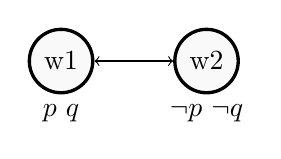
\begin{tikzpicture}[
				roundnode/.style={circle, draw=black, fill=gray!5, very thick, minimum size=7mm},
				]
		
					%Nodes
				\node[roundnode, label=below: $p \ q$]		(w1)				{w1};
				\node[roundnode, label=below: $\neg p \ \neg q$]		(w2)[right=of w1]	{w2};
		
				%Lines
				\draw[<->]	(w1.east) -- (w2.west);	
			\end{tikzpicture}
			&
			\begin{tabular}{c}
				$\square (p \rightarrow q)$ is \textsc{True} for $w_1$ and $w_2$ but $p \rightarrow \square q$ is \textsc{False} for $w_1$.
			\end{tabular}
		\end{tabular} \\
		Now we show that $p \rightarrow \square q \not \models \square (p\rightarrow g)$: \\
		\begin{tabular}{m{4.5cm} m{7.5cm}}
			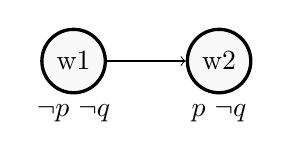
\begin{tikzpicture}[
				roundnode/.style={circle, draw=black, fill=gray!5, very thick, minimum size=7mm},
				]
		
					%Nodes
				\node[roundnode, label=below: $\neg p \ \neg q$]		(w1)				{w1};
				\node[roundnode, label=below: $p \ \neg q$]		(w2)[right=of w1]	{w2};
		
				%Lines
				\draw[->]	(w1.east) -- (w2.west);	
			\end{tikzpicture}
			&
			\begin{tabular}{c}
				$p \rightarrow \square q$ is \textsc{True} for $w_1$ and $w_2$ but $\square (p \rightarrow q)$ is \textsc{False} for $w_1$.
			\end{tabular}
		\end{tabular}
		
\end{document}